\chapter{Gravitational waves associated with gamma-ray bursts}\label{ch:grb}


\section{GW searches}\label{sec:grb-searches}

The \ac{LIGO}-Virgo collaboration searches for gravitational waves associated with \acp{GRB} detected by Fermi \ac{GBM} and Swift \ac{BAT} using two analyses: a template-based matched-filter search using the \pygrb pipeline and a generic transient search using \xpip~\citep{grb_o3a,grb_o3b}.
The \acp{GRB} are classified as short if $T_{90} + \abs{\delta T_{90}} < 2\,\text{s}$, long if $T_{90} - \abs{\delta T_{90}} > 4\,\text{s}$, and ambiguous if they lie in between.
The \pygrb pipeline is used for analyzing short and ambiguous \acp{GRB}, while \xpip is used for all \acp{GRB}, short, ambiguous or long.
This does not account for short GRBs that are followed by periods of extended emission, for which measures of $T_{90}$ may substantially exceed these thresholds.
For more robust classification one must also consider spectral properties, most commonly the spectral hardness or peak energy of the event, but since our sample consists of observations from multiple observatories with different spectral sensitivities we do not employ such quantities when organizing our sample.
The \acp{GRB} sample for a LIGO-Virgo observing run is collected from the Fermi and Swift \ac{GRB} catalogs, and the best sky localization and timing information is used.

\subsection{X-Pipeline}\label{sec:grb-x}

One of the analyses searching for \acp{GW} associated with \acp{GRB} uses the generic transient search library \xpip~\citep{Sutton_2010}.
This pipeline analyzes \ac{GW} strain data from multiple observatories around the time of a \ac{GRB}.
This is an unmodeled method for finding \acp{GW}, as it does not rely on template-based matched-filtering.
Instead, given a \ac{GRB} event, \xpip searches for excess power coherent between LIGO-Virgo detectors and consistent with the sky localization and time window of the \ac{GRB}.
The search time window starts 600\,s before the GRB trigger time and ends at 60\,s after trigger time, or at $T_{90}$ if $T_{90} > 60\,\text{s}$.
This is sufficient to cover the time delay between GW emission from a progenitor and any GRB prompt emission~\citep{Koshut_1995, Aloy_2000, MacFadyen_2001, Zhang_2003, Lazzati_2005, Wang_2007, Burlon_2008, Burlon_2009, Lazzati_2009, Vedrenne_2009}.
While some GW emissions, such as from \ac{CCSN}, are expected to reach frequencies up to a few kilohertz~\citep{Radice_2019}, we restrict our search frequency range to the most sensitive band of the GW detectors, 20–500\,Hz, since detecting such signals above a few hundred hertz requires extremely high GW energies~\citep{burst_o2} and expanding the frequency range would also significantly increase the computational cost. To constrain the sky location of the GRB event, the search uses a grid based on the best localization known either from Fermi \ac{GBM} or Swift \ac{BAT}.

Since \xpip is an unmodeled search, it primarily relies on coherence between detectors to determine the significance of a GW signal.
To do this, it combines the data from multiple detectors.
% To understand how this is done, consider the output of a single detector with antenna functions $F_+$ and $F_{\times}$ representing the sensitivity of the detector to GWs in the plus and cross polarizations, respectively, from a particular sky location.
% The detector response to a signal $h(t)$ with components $h_+$ and $h_{\times}$ is
% \begin{equation}
% 	d(t) = F_+ h_+(t) + F_{\times} h_{\times}(t) + n(t)
% \end{equation}
% where $n(t)$ is the background noise in the detector.
For a network of detectors, the data measured by a set of $D$ detectors is
\begin{equation}
	\mathbf{d} = \mathbf{F h} + \mathbf{n}
\end{equation}
where each component of the vectors $\mathbf{d}$ and $\mathbf{n}$ is the Fourier-transformed output of a detector and its noise, respectively,
\begin{equation}
	\mathbf{h} = \left( \begin{array}{c} h_+ \\ h_{\times} \end{array} \right)
\end{equation}
represents the plus and cross polarizations of the GW signal, and $\mathbf{F} = [\mathbf{F_+}\,\,\mathbf{F_\times}]$ is a matrix whose rows represent the antenna response of each detector to the plus and cross polarizations of the GW signal, respectively.
These matrix components are dependent on the sky location of interest, e.g. of a GRB trigger.
The components of $\mathbf{d}$, $\mathbf{n}$, and $\mathbf{F}$ are noise-spectrum-weighted, i.e. the raw value is divided by the one-sided noise power spectral density of the detector, such that $\mathbf{n}$ is normalized.
We refer to the noise-spectrum-weighted $\mathbf{d}$ as the energy measured in the detector.
We define the \textit{standard likelihood energy}
\begin{equation}\label{eq:grb-esl}
	E_{\mathrm{SL}} \equiv \sum_k^D \mathbf{d}^{\dagger} P^{\mathrm{GW}} \mathbf{d}
\end{equation}
where $P^{\mathrm{GW}} \equiv \mathbf{F} (\mathbf{F}^{\dagger} \mathbf{F})^{-1} \mathbf{F} \mathbf{F}^{\dagger}$ is a projection operator that projects the data into the subspace spanned by the antenna response vectors $\mathbf{F_+}$ and $\mathbf{F_\times}$.

To identify signals, \xpip Fourier transforms the individual detector streams over many time windows to produce time–frequency maps where each pixel represents the energy $d_k$ of detector $k$ for a particular time and frequency.
These maps give access to the temporal evolution of the spectral properties of the signal.
They are combined over the detector network via \cref{eq:grb-esl} to form a single map of pixels representing the standard likelihood energy.
Clusters are identified by selecting the 1\% of pixels with the highest standard likelihood energies and grouping together adjacent selected pixels.
Each cluster is assigned an overall detection statistic which is the sum of the standard likelihood energies of its pixels, and the cluster with the largest statistic is the best candidate for a GW detection.

The significance of a candidate is determined based on the probability of the event being produced by the background alone.
The data around the GRB trigger is divided into a 660\,s \textit{on-source} segment and many equally-long \textit{off-source} segments before and after the on-source.
The candidate significance is determined by comparing the \ac{SNR} of the trigger within the on-source segment to the distribution of the \acp{SNR} of the loudest triggers in the off-source segments.
As a requirement, the off-source segments are drawn from at least at least $\sim$1.5\,hr of coincident data from at least two detectors around the time of a \ac{GRB}.
This is small enough to select data where the detectors should be in a similar state of operation as during the \ac{GRB} on-source segment, and large enough so that statistical errors using artificial time-shifting of the data are at the sub-percent level.

We quantify the sensitivity of the generic transient search by injecting simulated signals into off-source data.
For each waveform family injected we determine the largest significance of any surviving cluster associated with the injections.
We compute the percentage of injections that have a significance higher than the best event candidate and look for the amplitude at which this percentage is above 90\%, which sets the upper limit.
We include O3b calibration errors~\citep{Acernese_2022, Sun_2021} by jittering the amplitude and arrival time according to a Gaussian distribution representative of the calibration uncertainties.
These injection sets allow us to calculate the 90\% exclusion distance, $D_{90}$, for each injection waveform.
These $D_{90}$ estimates represent the distance within which our null result is 90\% likely to exclude the existence of a \ac{GW} signal caused by the emission mechanism for that waveform.

We choose simulated waveforms to cover the search parameter space of three distinct sets of circularly polarized \ac{GW} waveforms: \ac{BNS} and \ac{NSBH} binary inspiral signals, stellar collapse signals, and disk instability signals.

\Ac{CSG} injections represent GW emission from stellar collapses defined in Equation (1) of~\citet{grb_o1} with a $Q$ factor of 9 and varying center frequency of 70, 100, 150, and 300\,Hz.
In all cases, we assume an optimistic emission of energy in \acp{GW} of $E_{\text{GW}} = 10^{-2} \msol c^2$.
This set of waveforms closely represents a number of emission models for short-duration \acp{GW} occurring during the collapse of the star.

Binary inspiral injections are chirp-like waveforms (similar to that of GW170817 as seen in Figure~\ref{fig:mma-gw170817}, top left).
They are generated based on masses sampled from a Gaussian distribution centered at 1.4\,$\msol$, with a width of 0.2\,$\msol$ for an \ac{NS} in a \ac{BNS} merger, and with a width of 0.4\,$\msol$ for an \ac{NS} in an \ac{NSBH} merger.
The distribution for \acp{GW} emitted by \ac{BNS} mergers addresses the case of short \ac{GRB} events as in~\citet{grb_o1} and adopted in the \pygrb search.

Long-duration \ac{ADI} injections are used to represent \acp{GW} produced by instabilities in the magnetically suspended torus around a rapidly spinning \ac{BH} formed by a massive core-collapsing star, as described in Section~\ref{sec:gw-grb-long}~\citep{vanPutten_2001, vanPutten_2004}.
Although the quadrupole mass moments within the torus can take on many forms, the waveforms used for the \xpip search are based on an approximation in which two overdense regions are formed on opposite sides of the torus and extract angular momentum from the central BH until the BH is no longer spinning, after which the lumps disperse and the torus returns to stability~\citep{Santamaria_2013}.
The spin-down produces GWs following a downwards-sweeping signal, different from the chirp that would be seen if the binary was simply spiraling inwards (Figure~\ref{fig:vanputten}).

\begin{figure}[h]
	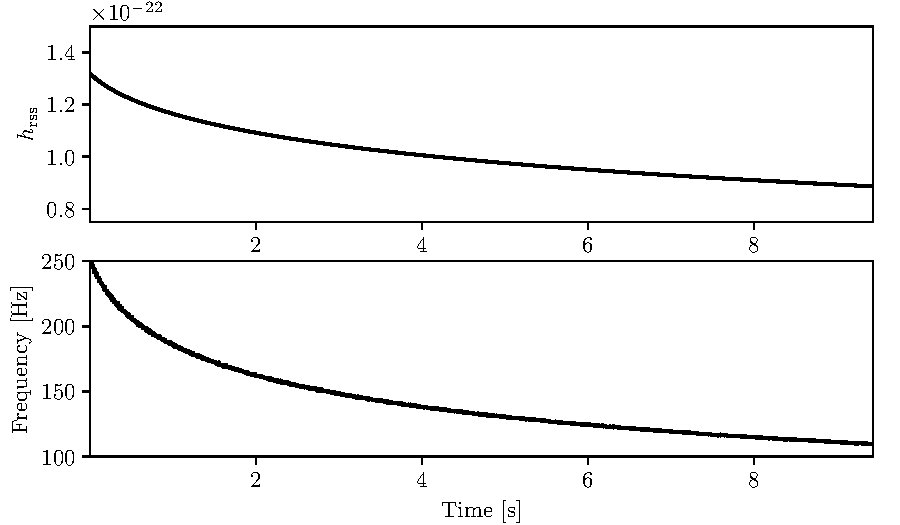
\includegraphics{figures/grb/vanputten.pdf}
	\caption{Example waveform of a ADI-B injection at 100\,Mpc. Parameters are given in Table~\protect\ref{tab:adi}.}
	\label{fig:vanputten}
\end{figure}

The ADI waveforms are parameterized by the mass $M$ and dimensionless spin parameter $\chi$ of the central \ac{BH}, and the fraction $\epsilon$ of the  accretion disk mass (which is fixed at $1.5\,\msol$) that forms into lumps.
The parameters used to generate the five families of \ac{ADI} signals are shown in Table~\ref{tab:adi}, along with the duration, frequency, and $E_{\text{GW}}$ of each waveform.

\begin{table}[h!]
	\centering
	\caption
  {Parameters and properties for accretion disk instability waveform injections.
  \label{tab:adi}}
	\begin{tabular}{c c c c c c c}
		\hline
		Waveform & $M$ ($\msol$) & $\chi$ & $\epsilon$ & Duration & Frequency & $E_{\text{GW}}$ \\
		Label &  &  &  & (s) & (Hz) & $(\msol c^2)$ \\
		\hline
  	\hline
    ADI-A & 5 & 0.30 & 0.050 & 39 & 135-166 & 0.02 \\
    ADI-B & 10 & 0.95 & 0.200 & 9 & 110-209 & 0.22 \\
    ADI-C & 10 & 0.95 & 0.040 & 236 & 130–251 & 0.25 \\
    ADI-D & 3 & 0.70 & 0.035 & 142 & 119–173 & 0.02 \\
    ADI-E & 8 & 0.99 & 0.065 & 76 & 111–234 & 0.17 \\
		\hline
	\end{tabular}
\end{table}


\subsection{Vetoing noise signals}

Combining the detector data streams coherently does not guarantee that chance coincidences between noise transients in the individual detectors cannot happen.
Before combining the data, \textit{data quality} (DQ) vetoes are applied to the single-detector signals.
DQ vetoes are observation periods flagged as problematic for various reasons.
Each detector has its own set of DQ vetoes, which are separated into different categories~\citep{Davis_2021, Davis_2021b}.
Category 1 DQ vetoes represent times during which detectors were not operating in their nominal state.
Many of these times correspond to large machines like forklifts and cranes being operated, for example.
Category 2 vetoes indicate periods where excess noise likely to be caused by known instrumental effects is present.
Examples from O3 include periodic 70\,Hz glitches caused by vibrations of a camera shutter at the LLO End-Y station, thunder noise identified by microphones at LLO during storms, and large earthquakes at LHO.
Category 3 flags are based on statistical correlations with auxiliary sensors.
Category 4 flags indicate times when hardware injections (signals intentionally generated in the interferometer to test search analyses or quantify correlations between the GW channel and auxiliary channels) were being performed.
The \xpip search completely removes times flagged by Category 1 vetoes before performing any analysis.
Category 2 and 4 flags are applied to the single-detector data streams prior to combining them.

After generating the coherent energy data stream and ranking the time-frequency pixel clusters, another step is taken by \xpip to further deal with non-astrophysical transients.
A coherent consistency test vetoes clusters based on the \textit{null energy} stream that is the difference between the total energy in the data $E_{\mathrm{tot}} = \sum_k \norm{d}^2$ and the standard likelihood energy defined in \cref{eq:grb-esl}:
\begin{equation}
	E_{\mathrm{null}} \equiv E_{\mathrm{tot}} - E_{\mathrm{SL}} = \sum_k^D \mathbf{d}^{\dagger} \mathbf{P}^{\textrm{null}} \mathbf{d}
\end{equation}
where $\mathbf{P}^{\textrm{null}} = (\mathbf{I} - \mathbf{P}^{\mathrm{GW}})$ is a projection operator orthogonal to $\mathbf{P}^{\mathrm{GW}}$ ($\mathbf{I}$ is the identity operator).
The null energy can be written as
\begin{equation}
	E_{\mathrm{null}} = \sum_k \sum_{\alpha, \beta} d_{\alpha}^{\dagger}  \mathbf{P}^{\textrm{null}}_{\alpha \beta} d_{\beta}
\end{equation}
which consists of cross-correlation terms ($\alpha \neq \beta$) and auto-correlation terms ($\alpha = \beta$).
The auto-correlation part is the \textit{incoherent energy}
\begin{equation}
	I_{\mathrm{null}} \equiv \sum_k \sum_{\alpha} \mathbf{P}^{\textrm{null}}_{\alpha \alpha} \norm{d_\alpha}^2
\end{equation}
which dominates $E_{\mathrm{null}}$ for a non-astrophysical signal.
Therefore $I_{\mathrm{null}} / E_{\mathrm{null}} \gg 1$ if a candidate is a GW and $I_{\mathrm{null}} / E_{\mathrm{null}} \simeq 1$ if it is a noise artifact.
The coherent consistency cut applies a threshold on this ratio, determined by a tuning procedure, and candidates falling below the threshold are vetoed.
Figure~\ref{fig:coh-cut} shows the results of this step being applied to the on-source segment of a GRB analysis.
The ratio cut is applied in this case about a factor of two above the diagonal, where $I_{\mathrm{null}} = E_{\mathrm{null}}$.

\begin{figure}[h]
	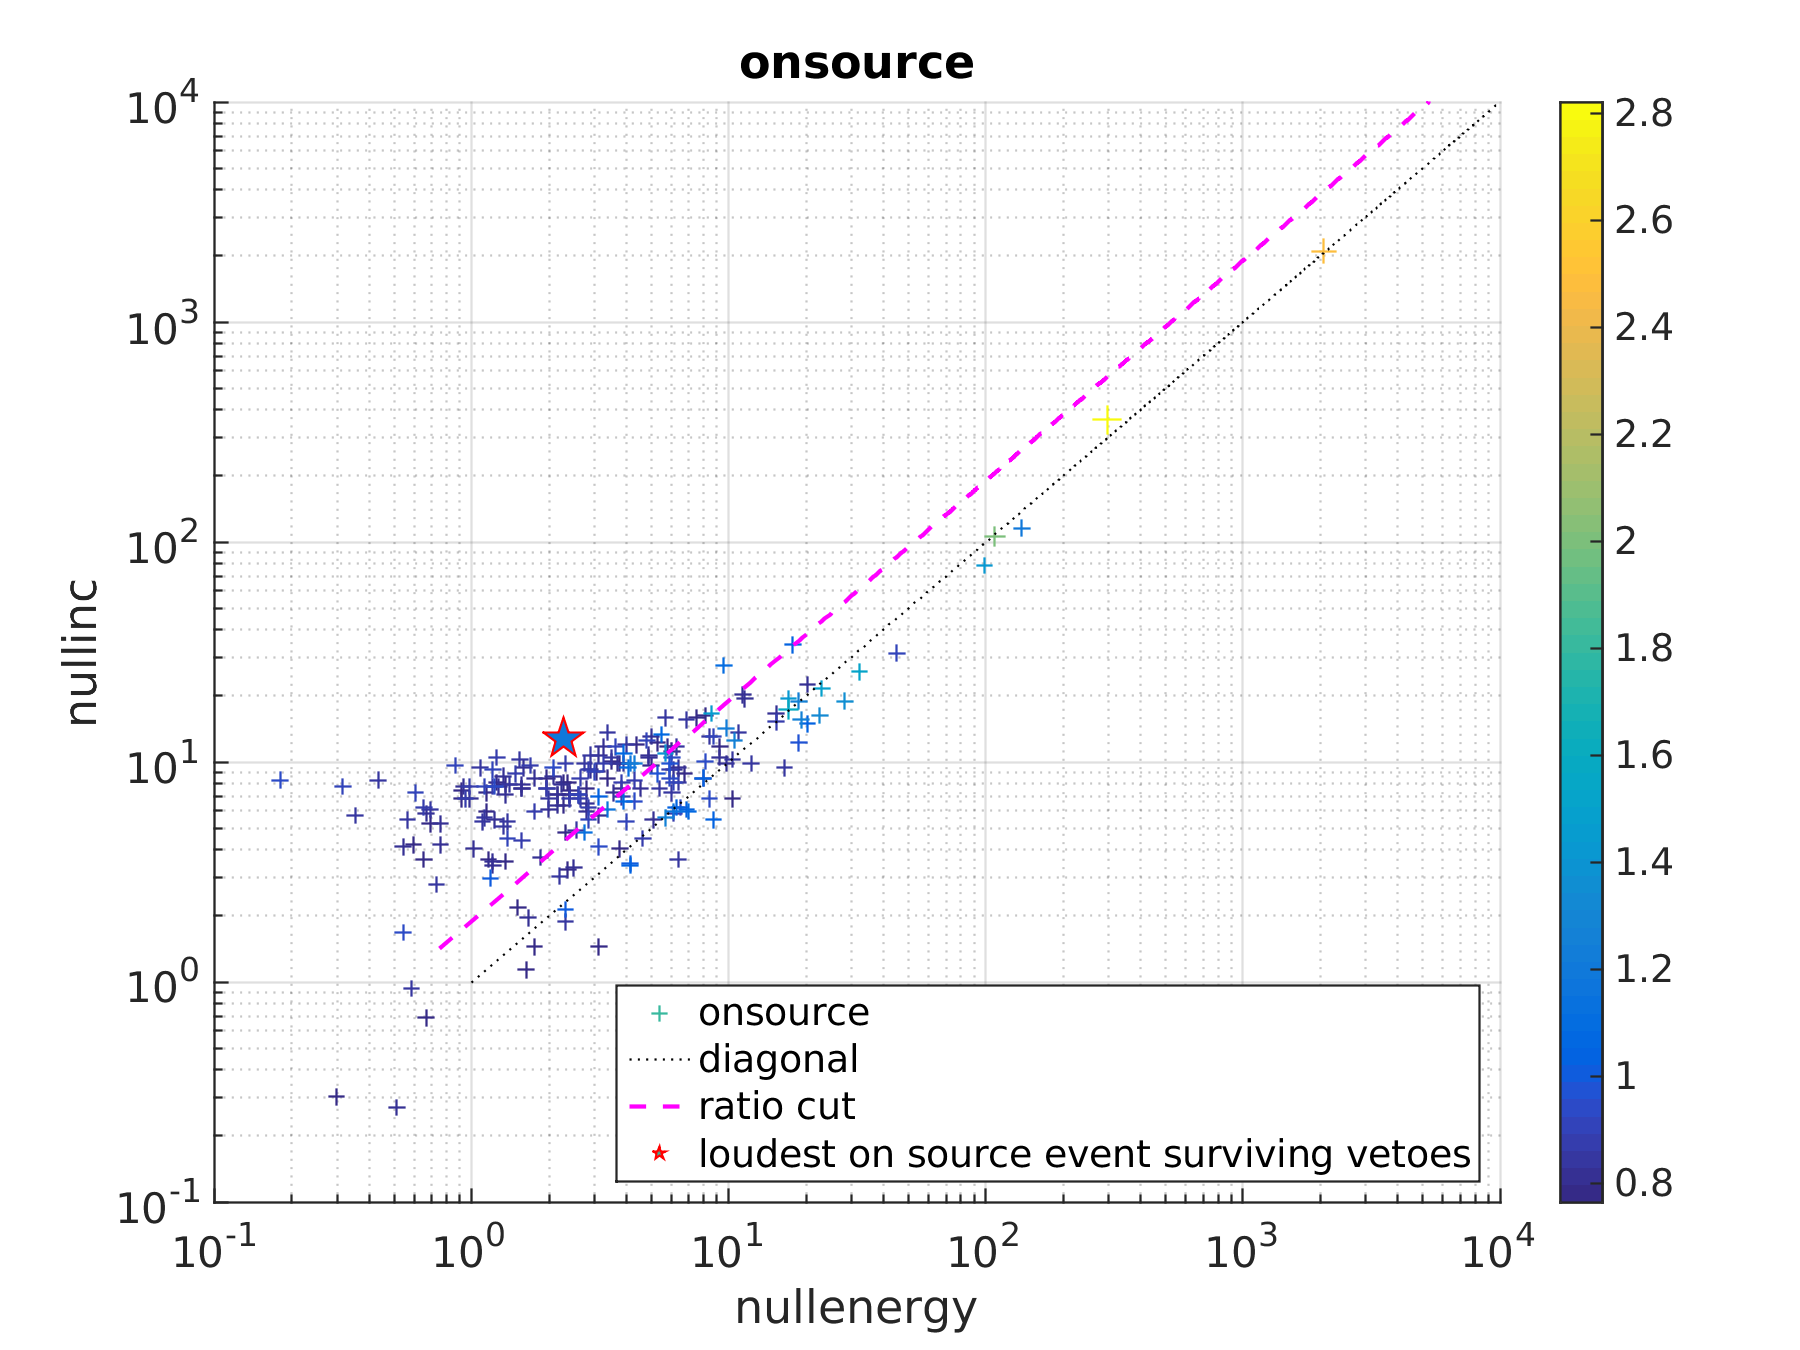
\includegraphics[width=0.8\textwidth]{figures/grb/coh-cut.png}
	\caption[Coherent consistency cut performed by \xpip to veto noise triggers.]{Coherent consistency cut performed by \xpip to veto noise triggers. The $x$- and $y$-axes represent $E_{\mathrm{null}}$ and $I_{\mathrm{null}}$, respectively.}
	\label{fig:coh-cut}
\end{figure}

In the O3a search, the sensitivity to long-duration ($\geq 10\,\text{s}$) GW signals was often limited by loud background noise transients.
While the coherent consistency tests easily veto these glitches, many long-duration simulated signals would overlap such a glitch by chance.
In these cases the simulated signal and glitch would be clustered together and subsequently vetoed together.
To address this problem, an ``autogating'' procedure was implemented for O3b. For each detector, the total energy in the whitened data stream is computed over a 1\,s window.
If this total fluctuates by more than 50 standard deviations above the median value, then the data is zeroed out over the interval where the threshold is exceeded.
A 1\,s inverse Tukey window is applied at each end of the zeroed interval to transition smoothly between the whitened and zeroed data.
To minimize the possibility of a loud GW transient triggering a gate, the procedure cancels a gate if there is a simultaneous energy excursion above 10 standard deviations in any other detector.
The threshold of 50 standard deviations is low enough to gate the most problematic loud glitches, while being high enough that the only GWs zeroed out by the gate would have been detectable by all-sky searches.
Empirically we find that this procedure is effective at reducing the impact of loud glitches without affecting the sensitivity to low-amplitude GW signals.


\section{O3b search for GWs associated with GRBs}\label{sec:grb-o3b}

Since \ac{O3} was split into two halves, O3a and O3b, the \ac{LIGO}-Virgo \ac{GRB} search was also split in two~\citep{grb_o3a,grb_o3b}.
The main differences in O3b where changes in the detector during the in-between commissioning phase resulted in improvements to the sensitivity of the LIGO detectors, and as mentioned above the autogating algorithm was introduced.

The full sample of \acp{GRB} occurring in O3b consists of seven short \acp{GRB}, 12 ambiguous \acp{GRB}, and 89 long \acp{GRB}.
Of these, only two have known redshifts: GRB 191221B ($z = 1.148$)~\citep{Kuin_2019, Vielfaure_2019} and GRB 200205B ($z = 1.465$)~\citep{Vielfaure_2020}.
Since \xpip searches for coincident excess power, we perform the generic transient search for \acp{GRB} where at least two of the three LIGO-Virgo detectors were active.
This leads to 86 GRBs to analyze and is also compatible with the network observing time of at least two detectors (85.3\%).

Running \xpip produces a ``closed-box'' results page, which summarizes the results of the search on a ``dummy'' on-source window chosen from among the off-source windows.
This allows us to tune the parameters of the search, the injections, or the pre- and postprocessing to produce the most sensitive closed-box results before actually analyzing the on-source data (the ``open-box'' analysis).
We first analyze each \ac{GRB} \textit{without} autogating, and rerun the closed-box analysis \textit{with} autogating only if the initial closed box results suggest that autogating would improve the sensitivity of the search.
The glitches targeted by autogating affect the ability of \xpip to detect long-duration signals, so we can determine if a closed-box analysis would perform better with autogating applied by looking for a clear plateau or dip in the detection efficiency curves of the long-duration \ac{ADI} waveforms, accompanied by signs of high-energy triggers in diagnostic figures produced in the results page.
If such a problem does exist, then the closed-box analysis is rerun with autogating, and the box with better efficiency curves (usually the autogated version) is opened.
Otherwise, if autogating is not likely to affect the results, then we open the initial non-autogated box.

As an example of this procedure, we will consider the analysis of GRB191101A, an extreme case of noisy background data.
This is a long GRB observed by Swift during which LHO, LLO, and Virgo were all active.
Figure~\ref{fig:gauss-before} shows the Gaussianity measures for the three detectors (LHO, LLO, and Virgo represented as H1, L1, and V1).
The Gaussianity measures represent the ratios between the variance of the detector spectra to their means; high values correspond to high deviations from Gaussian behavior.
The low-frequency excess is likely associated with scattered light noise, whereas the flat component is typical of the broadband glitches that autogating is designed to combat.
The LHO and Virgo measures, meanwhile, lie within the normal levels of non-Gaussianity, shown by the black dashed lines at the bottom of the figure.

\begin{figure}[htb]
	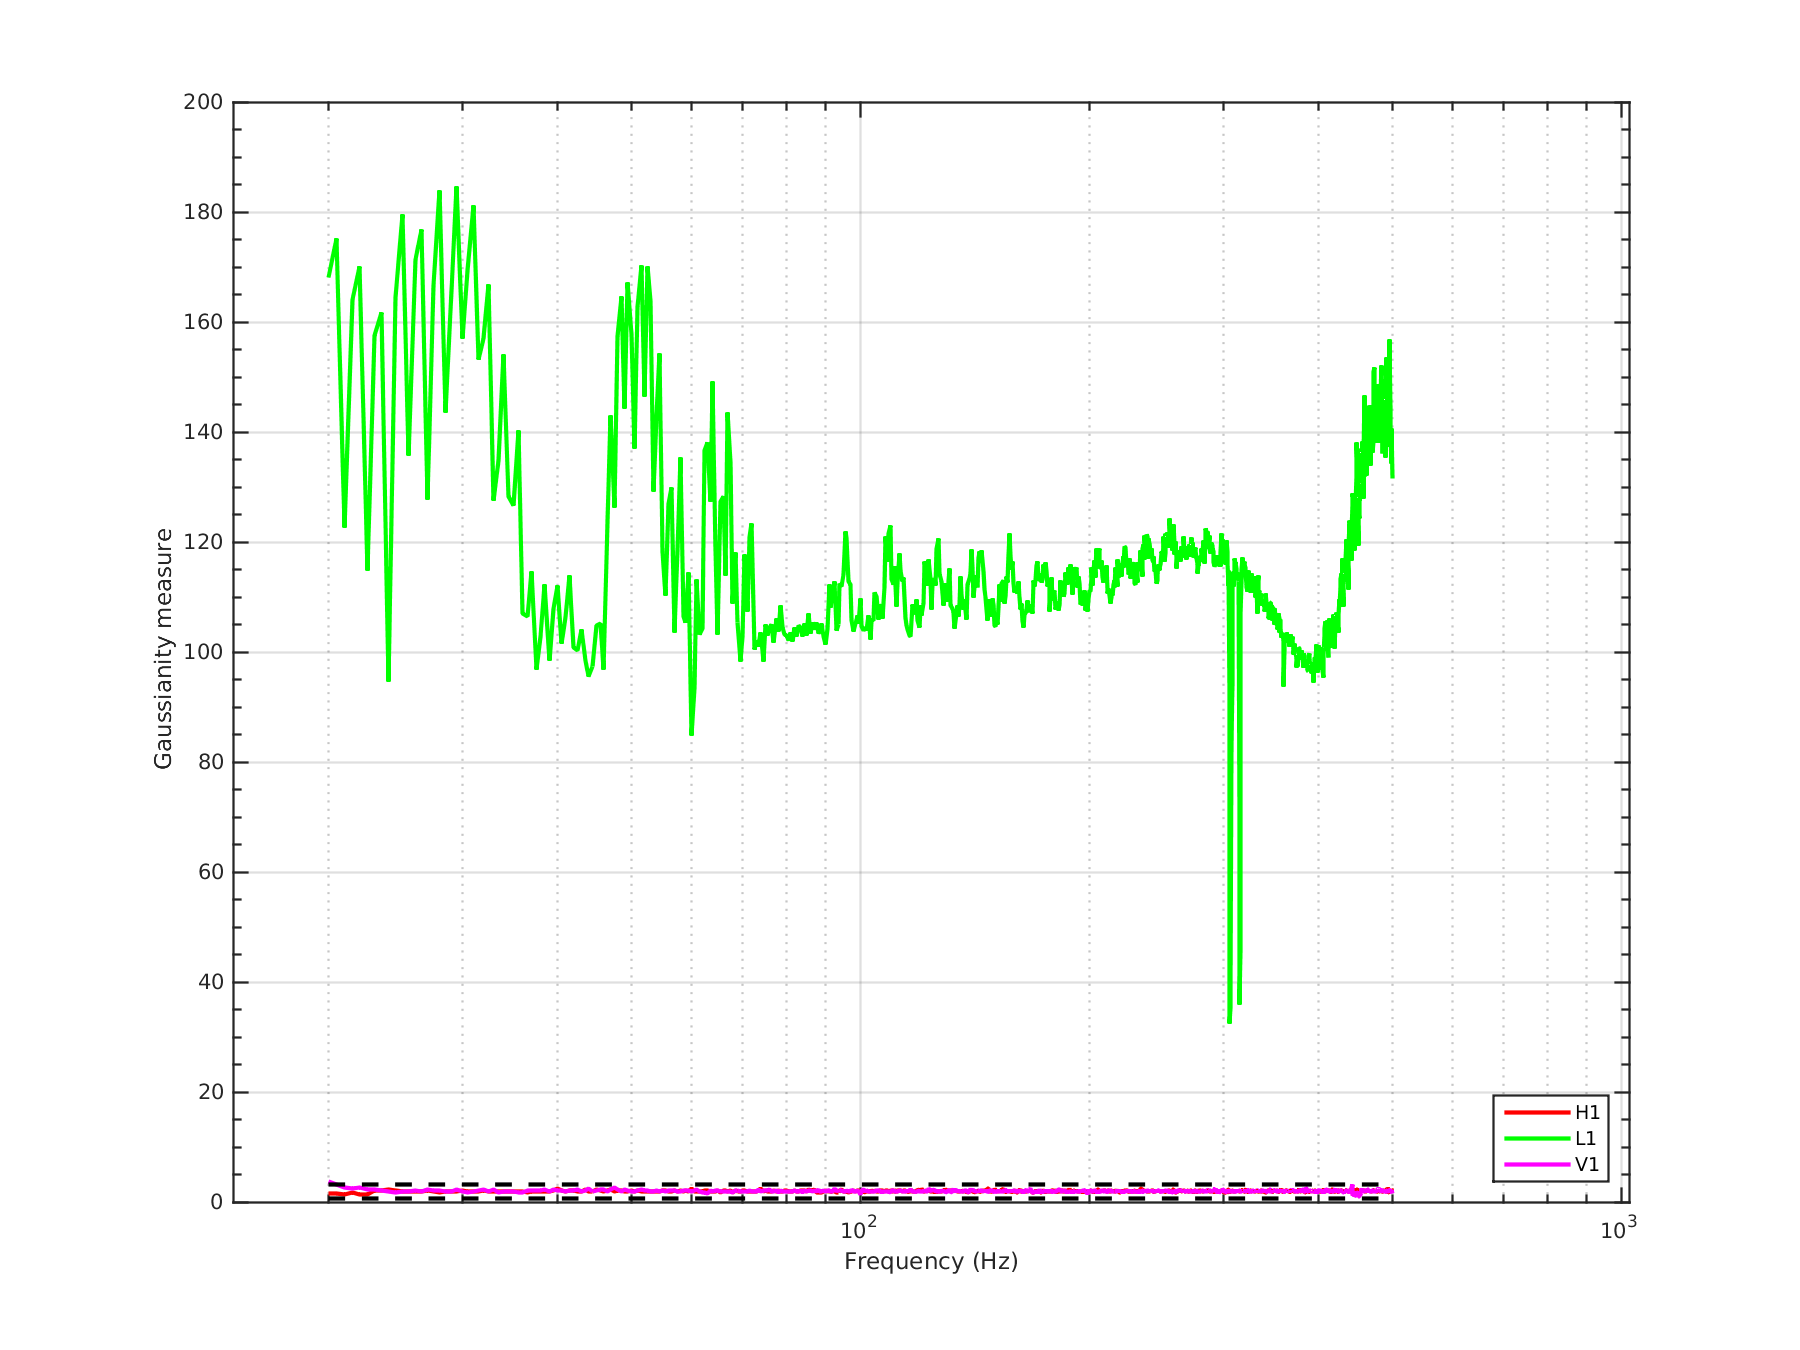
\includegraphics[trim={2cm 1.2cm 2cm 1.5cm}, clip, width=\textwidth]{figures/grb/gauss-before.png}
	\caption[Gaussianity measures around the time of GRB191101A without autogating.]
	{Gaussianity measures around the time of GRB191101A without autogating. The black horizontal dashed lines represent the expected levels of non-Gaussianity. LHO (H1) and Virgo (V1) are both within these bounds, while LLO (L1) far exceeds them.}
	\label{fig:gauss-before}
\end{figure}

Figure~\ref{fig:triggers-before} shows the distribution of triggers in LLO and LHO after applying data quality vetoes but before applying coherent consistency vetoes.
The most problematic glitches appear as triggers with energies in the tens of thousands.
They make up a small minority of all the triggers, but their impact on the pipeline's ability to detect injected signals is tremendous.

\begin{figure}[htb]
	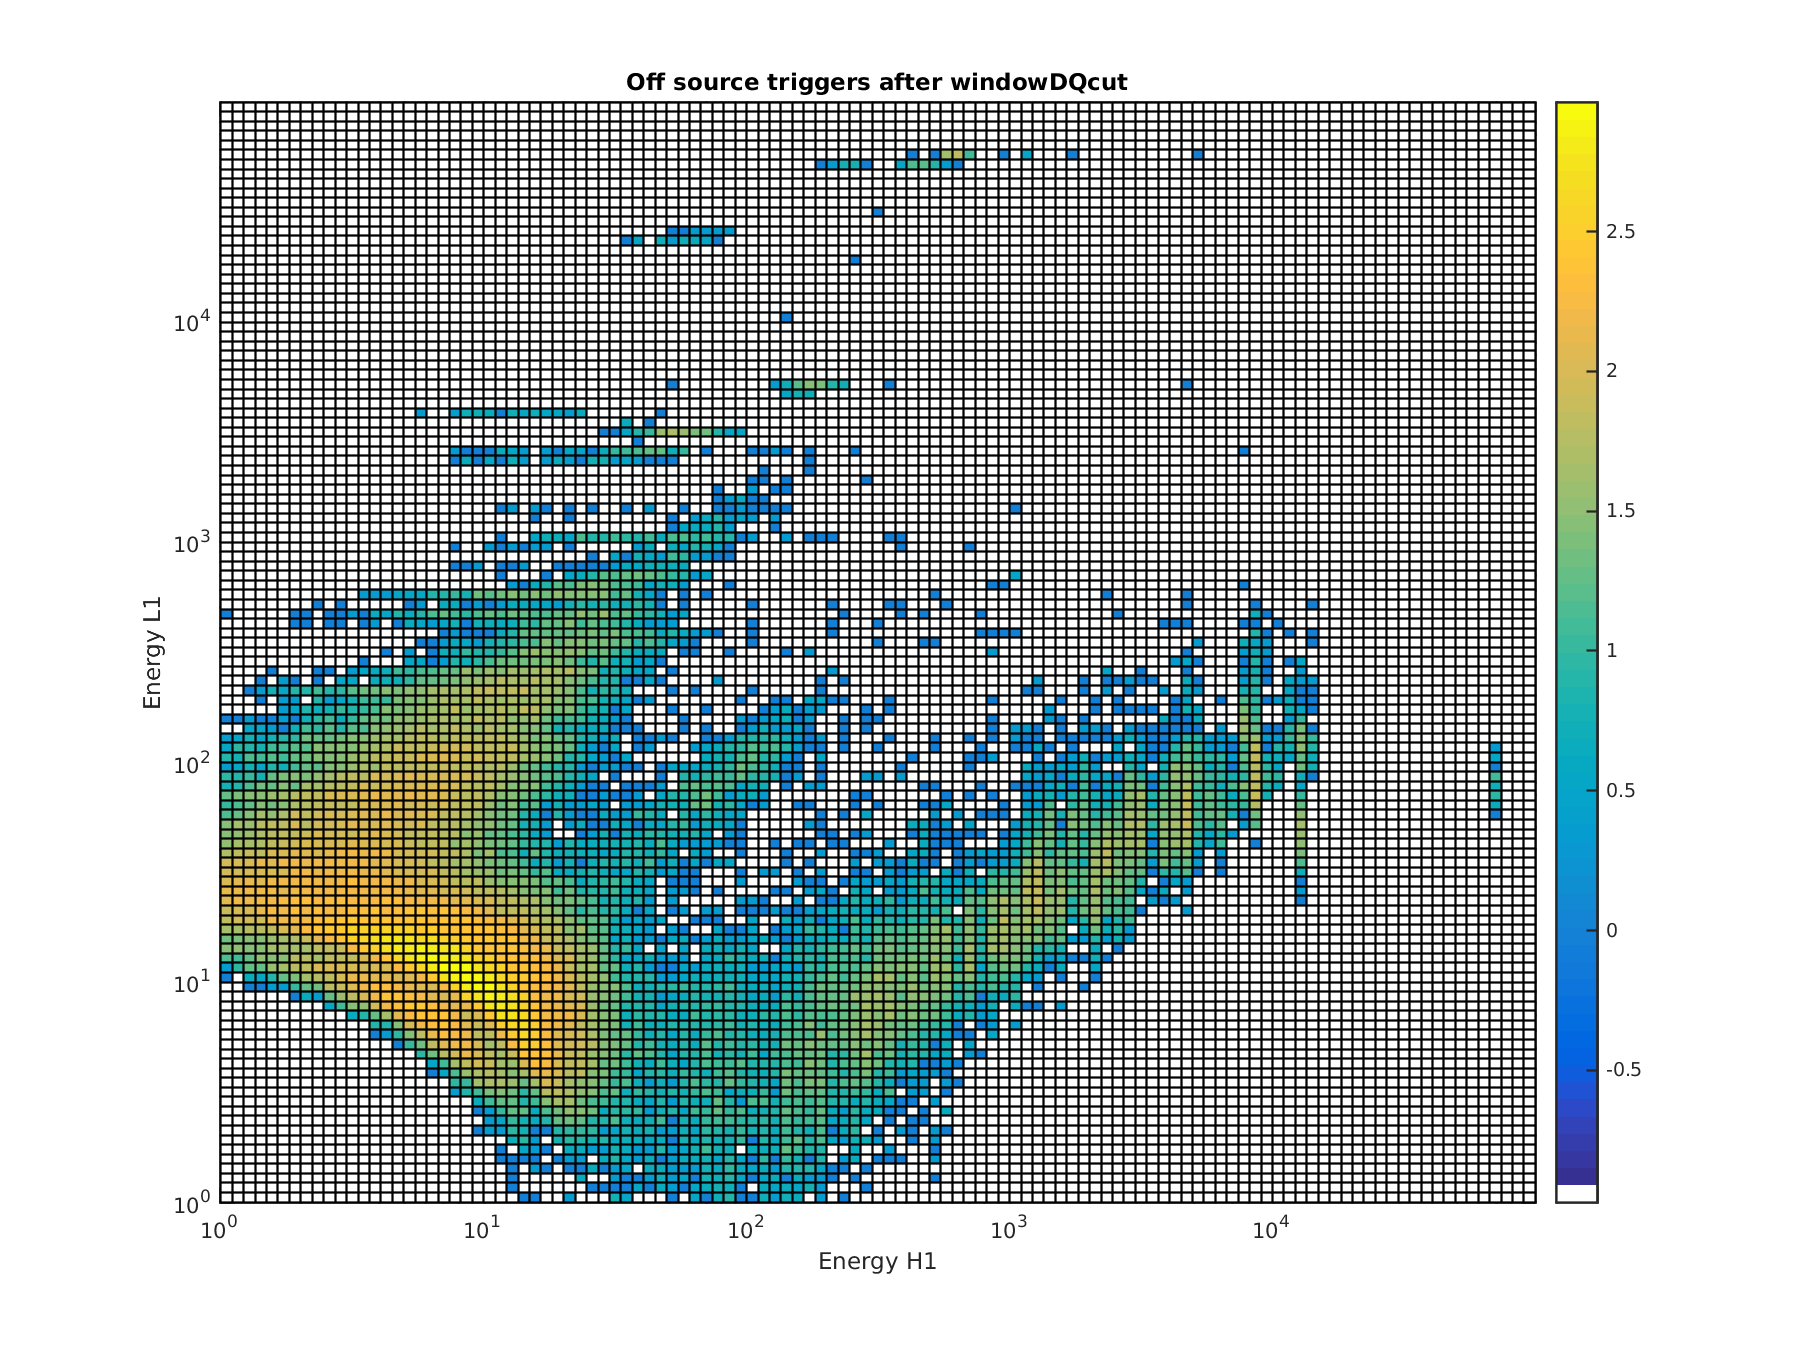
\includegraphics[trim={2cm 1.2cm 2cm 1.2cm}, clip, width=0.9\textwidth]{figures/grb/triggers-before.png}
	\caption{Distribution of off-source triggers in the LIGO detectors without autogating. The x- and y-axes are the signal energy in H1 and L1, respectively.}
	\label{fig:triggers-before}
\end{figure}

Figure~\ref{fig:eff-before-after} shows a major dip in the detection efficiency for a long-duration injection, ADI-C, when autogating is not applied.
The dip is entirely fixed with autogating active, leaving only a small, acceptable plateau in the efficiency curve around 95\%.

\begin{figure}[htb]
	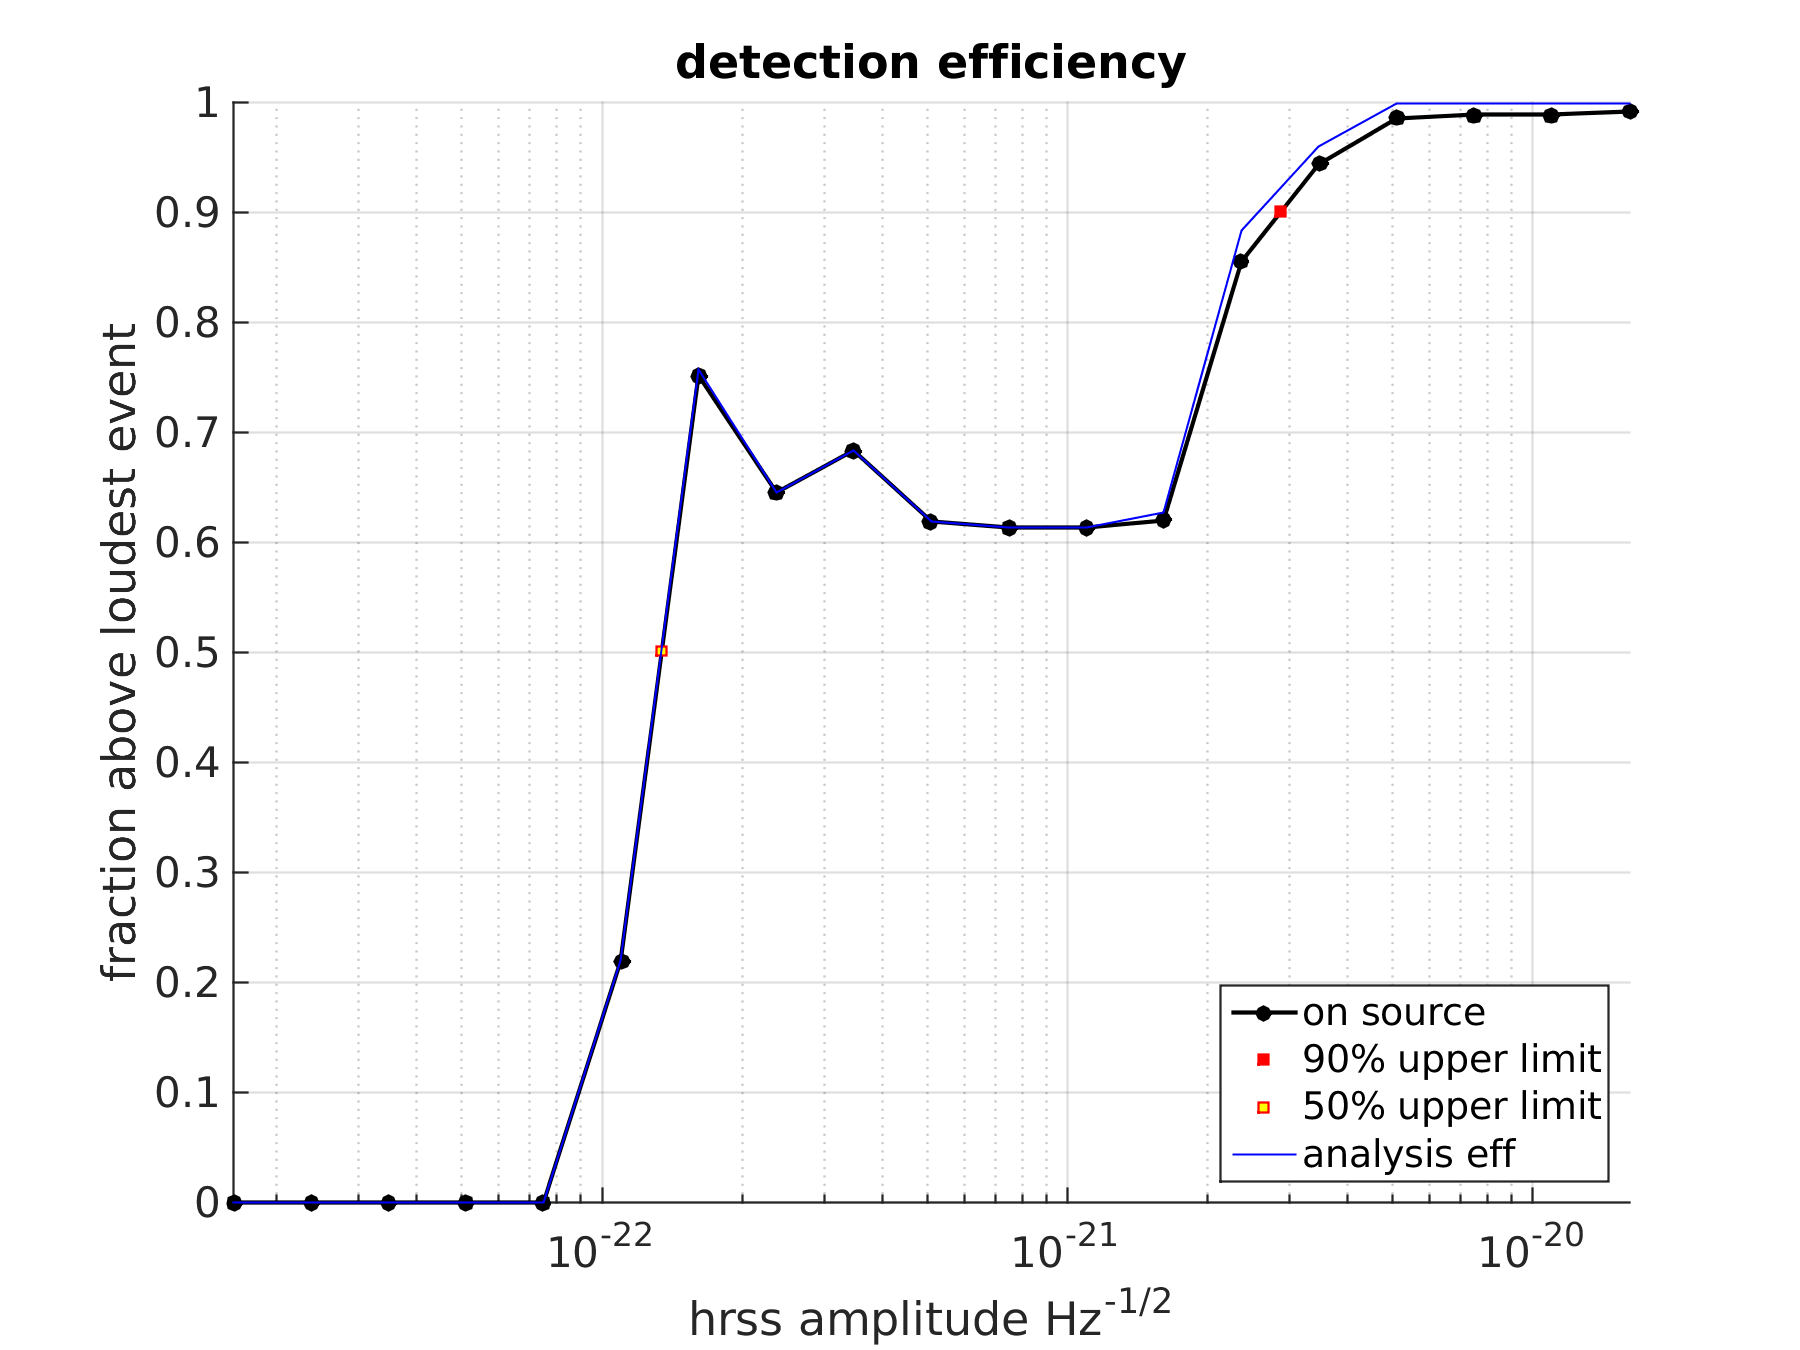
\includegraphics[trim={1.1cm 0 1.6cm 0}, clip, width=0.5\textwidth]{figures/grb/eff-before.png}
		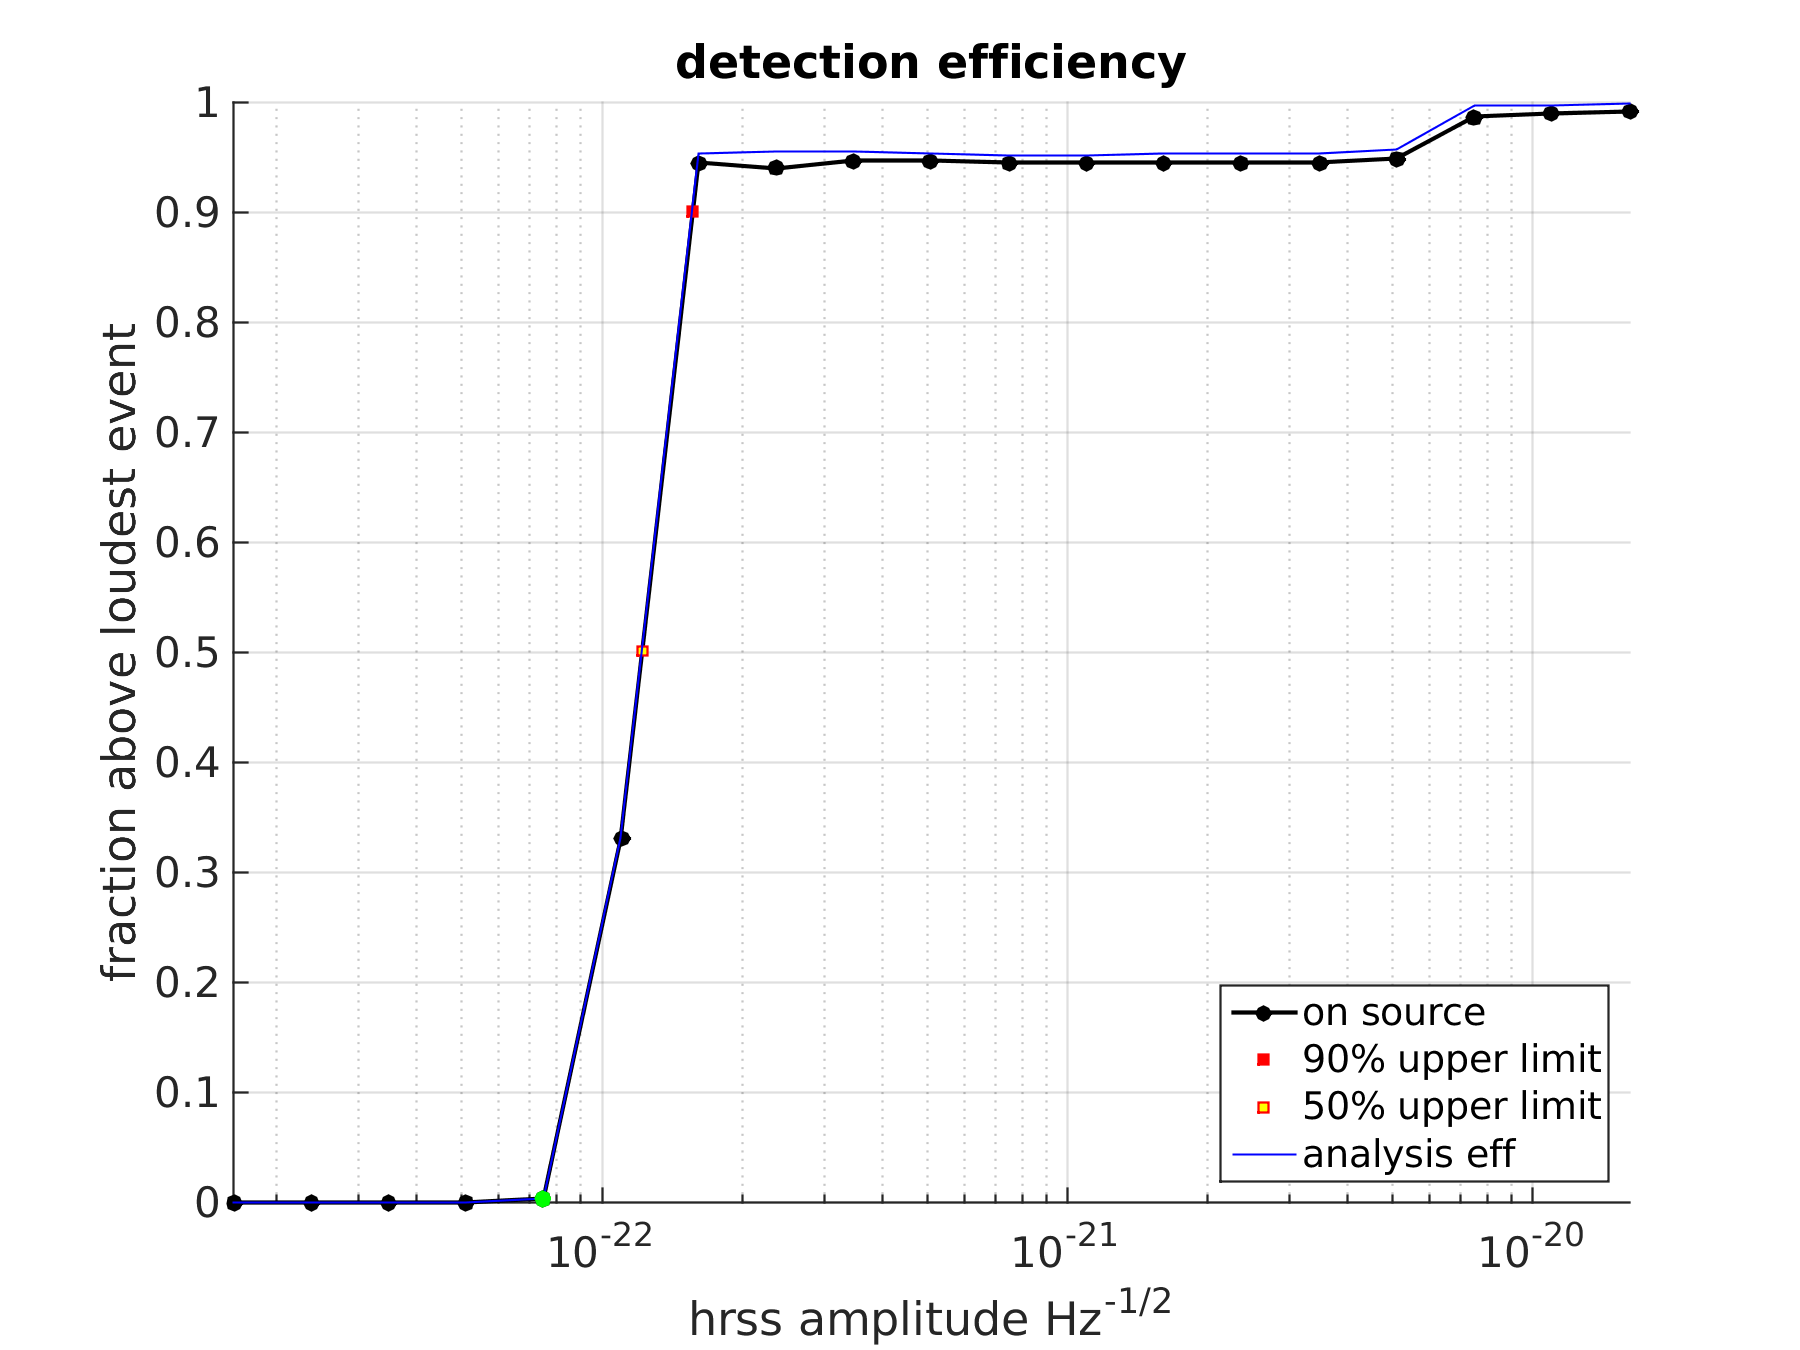
\includegraphics[trim={1.1cm 0 1.6cm 0}, clip, width=0.5\textwidth]{figures/grb/eff-after.png}
	\caption{Detection efficiency of ADI-C injected waveforms without (left) and with (right) autogating.}
	\label{fig:eff-before-after}
\end{figure}

% \begin{figure}[htb]
% 	\includegraphics[trim={2cm 1.2cm 2cm 1.2cm}, clip, width=\textwidth]{figures/grb/triggers-after.png}
% 	\caption{Distribution of off-source triggers in the LIGO detectors with autogating.}
% 	\label{fig:triggers-after}
% \end{figure}

% \begin{figure}[htb]
% 	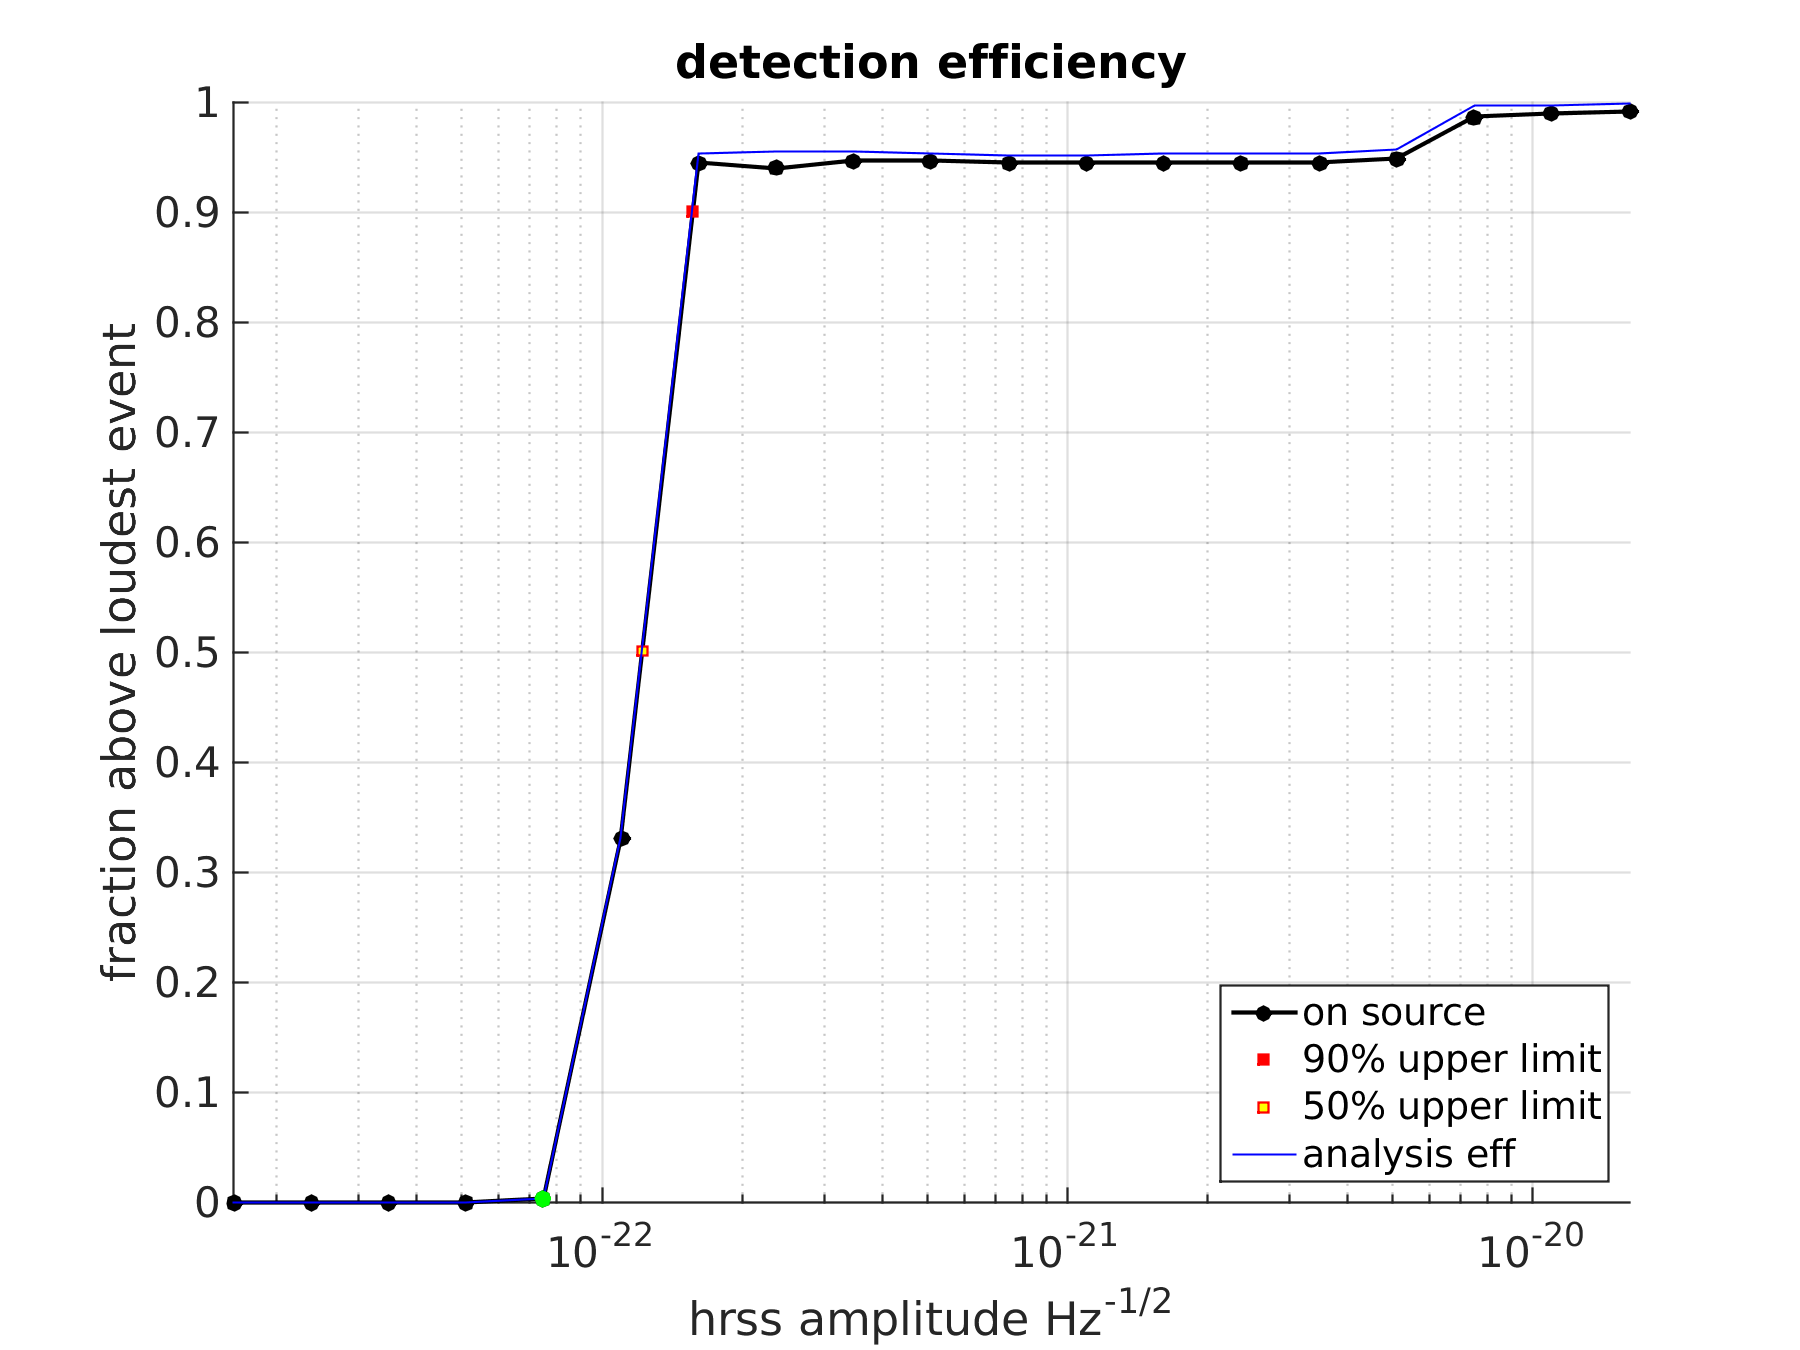
\includegraphics[trim={1cm 0 1.5cm 0}, clip, width=\textwidth]{figures/grb/eff-after.png}
% 	\caption{Detection efficiency of ADI-C injected waveforms with autogating.}
% 	\label{fig:eff-after}
% \end{figure}

Ultimately, autogating was performed on more than half of the 86 O3b GRB triggers analyzed by \xpip.
This seems to suggest that it would be better to have autogating active by default, but it is not clear from an autogated closed box result page if it was needed in the first place.
Therefore it is recommended that in future searches we continue to run \xpip without autogating first and only apply it when needed.
Even though the negative trade-off of autogating (reducing detection efficiency for very high amplitude signals) is not too concerning, keeping the analysis as simple as possible may be a preferable route.
Nevertheless, this will have to be weighed against the greater computing time spent for autogating reruns, since having to rerun most of the closed box analyses roughly doubles the amount of time before final results are produced.


\subsection{Results of the O3b search}\label{sec:grb-o3b-results}

We rank each candidate by calculating a p-value, the probability of an event or a louder one in the on-source data, given the background distribution, under the null hypothesis.
The p-value is calculated by counting the fraction of background trials that contain an event with a greater signal-to-noise ratio than that of the loudest on-source event.
Figure~\ref{fig:grb-o3b-x-pval} shows the distribution of p-values for the 86 \acp{GRB} analyzed by \xpip.
In this plot, a significant event would appear at a much lower p-value in the lower left corner of the plots, and be outside (to the left) of the 90\% confidence region.
The plot shows that the p-value distribution is consistent with the background.
The lowest reported p-value found during O3b for the generic transient search was $7.95\times 10^{-3}$ (GRB 200224B). Although this p-value is very small, it is not unexpected given the high number of GRBs analyzed.

\begin{figure}[h]
  \centering
  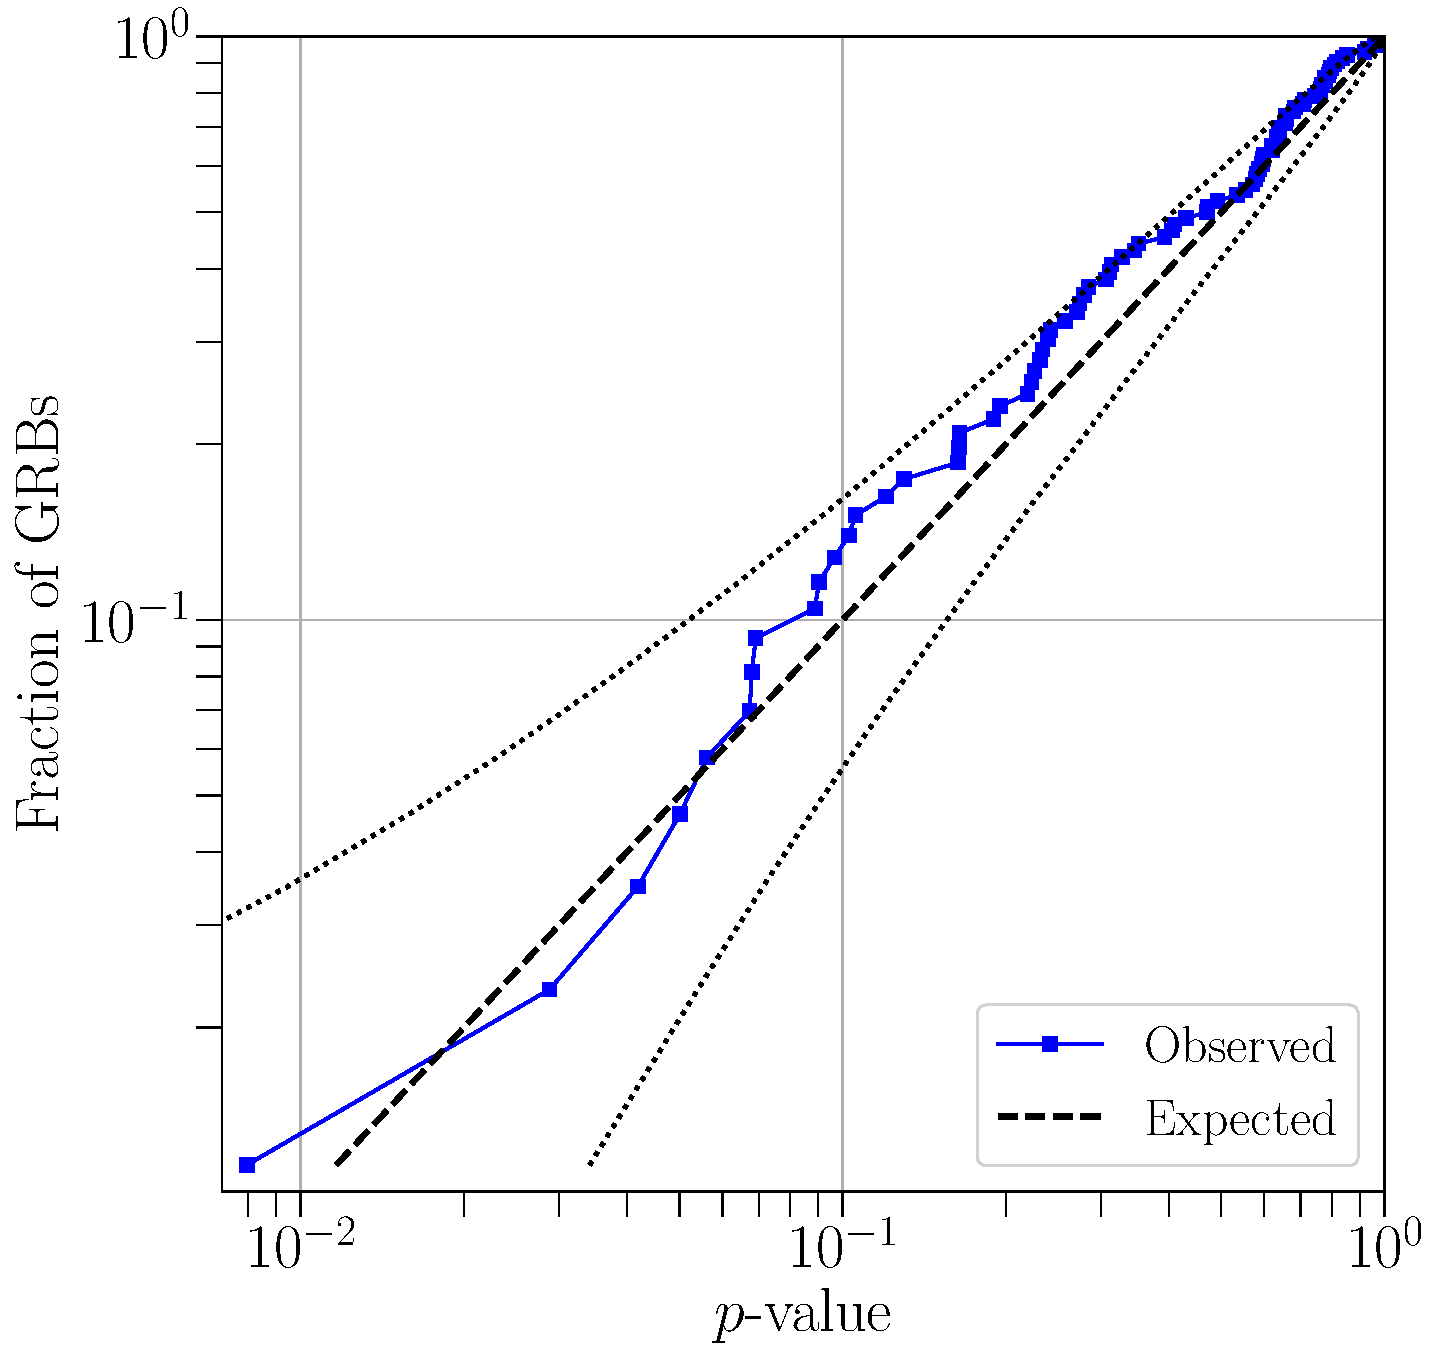
\includegraphics[width=0.7\textwidth]{figures/grb/o3b-x-pval.pdf}
  \caption
  [Cumulative distribution of p-values for the loudest on-source events of the O3b X-pipeline analyses.]
  {
    Cumulative distribution of p-values for the loudest on-source events of the O3b X-pipeline analyses.
    The dashed line indicates an expected uniform distribution of p-values under a no-signal hypothesis, with the corresponding 90\% band as the dotted lines.}
  \label{fig:grb-o3b-x-pval}
\end{figure}

Given that no loud \ac{GW} signals are observed coincident with any of the \acp{GRB} in this search, we perform a weighted binomial test to determine the probability of observing our set of p-values assuming a uniform background distribution~\citep{grb_s4, grb_s6}.
A small probability would suggest that there may be a population of subthreshold \ac{GW} signals that our search did not identify.
This type of weighted binomial test uses the lowest re-weighted p-values from the searches.
For the generic transient search, the test gives a probability of 0.76.
The same test carried out in O3a returned a probability of 0.30~\citep{grb_o3a}.
In O2 (removing GW170817/GRB 170817A) and O1 the probabilities were 0.75 and 0.75, respectively~\citep{grb_o2, grb_o1}.
As in these previous analyses, the probabilities obtained in O3b suggest that no weak GW sources can be attributed to the population of GRBs.

\begin{figure}[h]
  \centering
  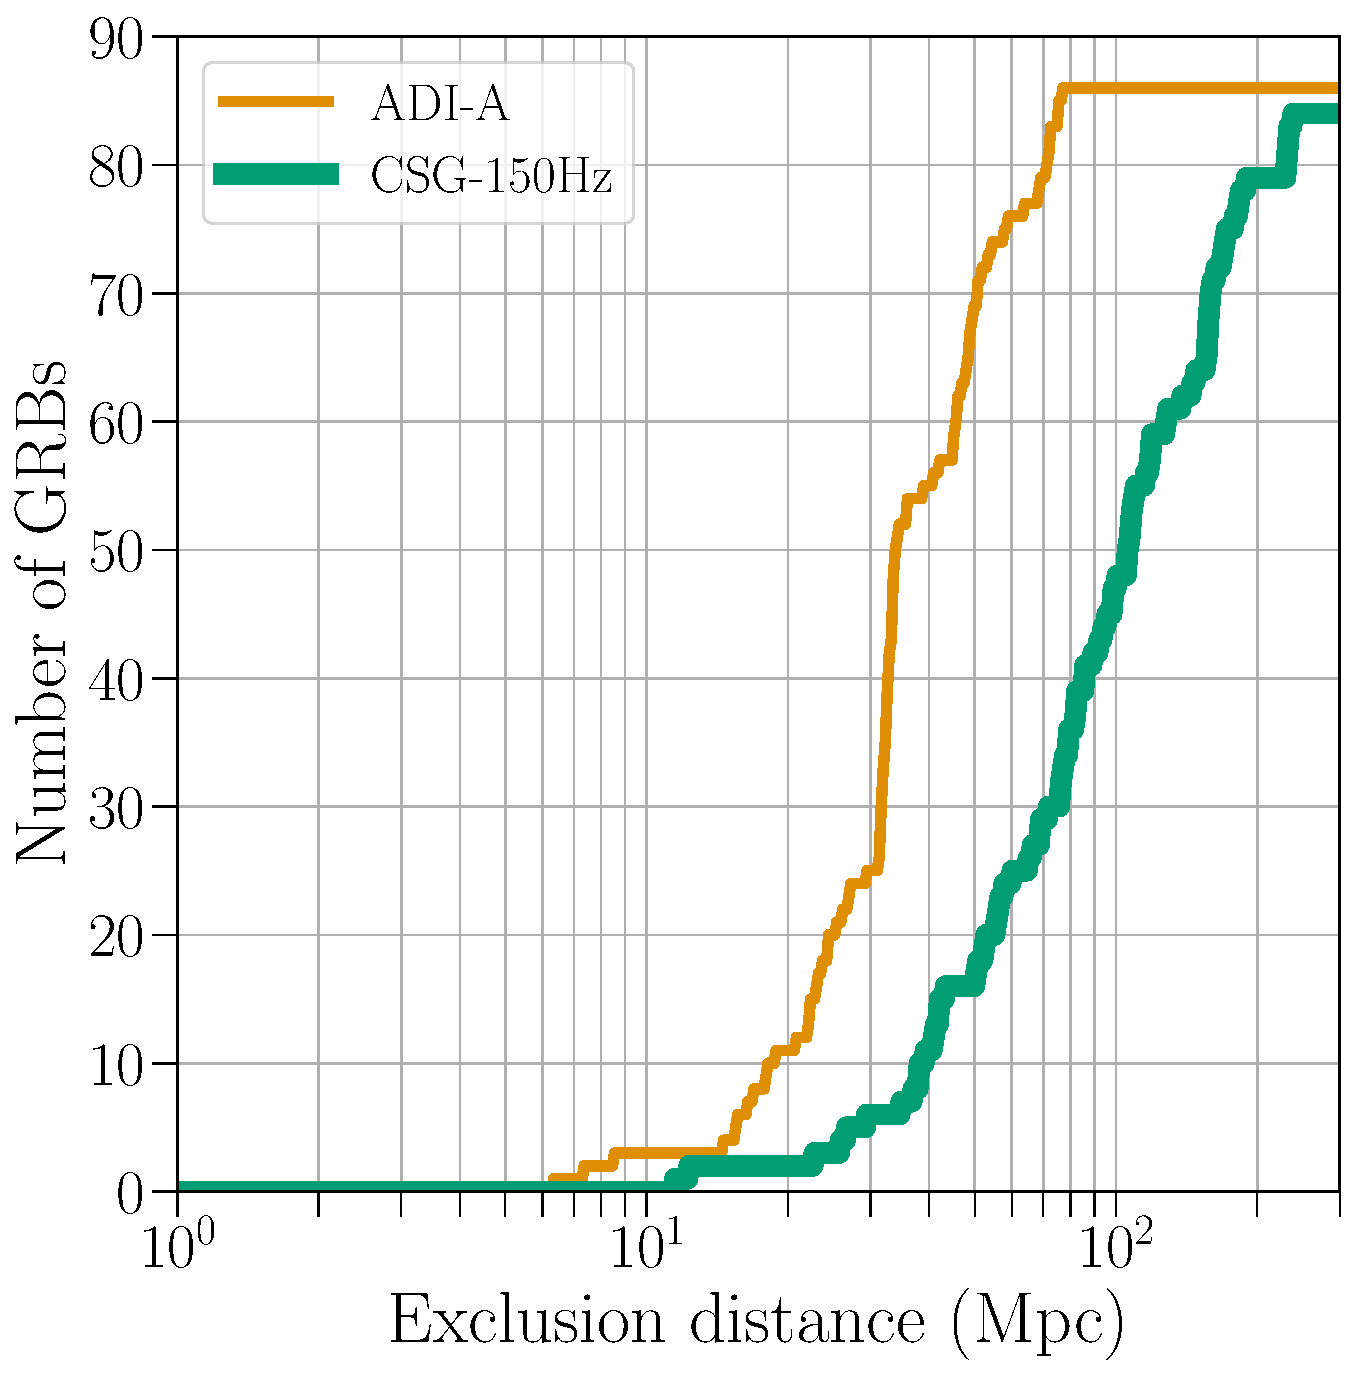
\includegraphics[width=0.7\textwidth]{figures/grb/o3b-x-exclusion.pdf}
  \caption{Cumulative distributions of O3b exclusion distances for 150-Hz sine-Gaussian and ADI-A waveforms.}
  \label{fig:grb-o3b-x-exclusion}
\end{figure}

We derive a 90\% confidence level lower limit on the distance for each of the 86 GRBs analyzed with the generic transient search, based on the different emission models.
Figure~\ref{fig:grb-o3b-x-exclusion} shows the distribution of $D_{90}$ values for the ADI-A model and for a CSG with central frequency of 150\,Hz.
The limits reported depend on the sensitivity of the instruments in the network, which change with time and sky localization of the GRB events.
We marginalize these limits over errors introduced by detector calibration.
Table~\ref{tab:grb-o3b-x-exclusion} reports the median $D_{90}$, for the set of GRBs for the different signals.
The limits vary by nearly an order of magnitude due to the variety of signals used in our analysis.
On average, the median values for the O3b generic transient search are about 50\% greater than those reported in O3a~\citep{grb_o3a}.

\begin{table}[h]
  \hspace{0.5cm}
  \caption
  {\label{tab:grb-o3b-x-exclusion} Median 90\% exclusion distances ($D_{90}$) for the generic transient search during O3b.}
  \begin{tabular}{c c c c c}
    \hline
    \hline
    \rule{0pt}{4ex}
    & CSG 70\,Hz & CSG 100\,Hz & CSG 150\,Hz & CSG 300\,Hz \\
    \hline
    \rule[-2ex]{0pt}{4ex}
    $D_{90}$ [Mpc] & 166 & 126 & 92 & 42
  \end{tabular}
  %
  \begin{tabular}{c c c c c c}
    \hline
    \hline
    \rule{0pt}{4ex}
    & ADI-A & ADI-B & ADI-C & ADI-D & ADI-E \\
    \hline
    \rule[-2ex]{0pt}{4ex}
    $D_{90}$ [Mpc] & 34 & 140 & 54 & 22 & 52 \\
    \hline
  \end{tabular}
\end{table}


\subsection{Noise effects in the generic transient search}\label{sec:grb-o3b-noise}

Comparing the exclusion distances of the O3a and O3b search sheds some light on the impact of detector and search pipeline improvements on the sensitivity of the \xpip analysis.
Table~\ref{tab:grb-o3b-compare-o3a} presents the improvement in the median $D_{90}$ for each waveform model as a fraction of the O3a value.
The exclusion distances for the shorter-duration CSG waveforms, which are not expected to be affected by autogating, increased by about 30\% on average.

\begin{table}[h]
  \hspace{0.5cm}
  \caption
  {\label{tab:grb-o3b-compare-o3a} Relative increase in median $D_{90}$ for each \xpip simulated waveform.}
  \begin{tabular}{c c c c c}
    \hline
    \hline
    \rule{0pt}{4ex}
    & CSG 70\,Hz & CSG 100\,Hz & CSG 150\,Hz & CSG 300\,Hz \\
    \hline
    \rule[-2ex]{0pt}{4ex}
		$\Delta D_{90} / D_{90, \text{O3a}}$ & 0.12 & 0.19 & 0.25 & 0.49
  \end{tabular}
  %
  \begin{tabular}{c c c c c c}
    \hline
    \hline
    \rule{0pt}{4ex}
    & ADI-A & ADI-B & ADI-C & ADI-D & ADI-E \\
    \hline
    \rule[-2ex]{0pt}{4ex}
    $\Delta D_{90} / D_{90, \text{O3a}}$ & 0.43 & 0.14 & 0.85 & 0.92 & 0.55 \\
    \hline
  \end{tabular}
\end{table}

Given the large number of GRBs analyzed, it would be unlikely for the difference to be explained by chance improvement in antenna response (i.e. due to more GRBs lining up with the sky region where the GW detector network is most sensitive).
\xpip reports the antenna response of the GW detectors for each GRB analyzed.
These can be summed up over the active detectors for each GRB and averaged over the full GRB sample.
The result is a 9.2\% improvement in antenna response, which is not negligible but can only account for a small portion of the differences in exclusion distances.

For the longest duration ADI-C, ADI-D, and ADI-E waveforms, we see the greatest improvements, over 50\% higher than in O3a (Figure~\ref{fig:grb-o3b-compare-o3a}, top).
For short-duration waveforms, the highest-frequency 300-Hz sine-Gaussian injections show the greatest change (Figure~\ref{fig:grb-o3b-compare-o3a}, bottom).
These are all well above the change expected from a chance difference in antenna response.

\begin{figure}[h]
  \centering
  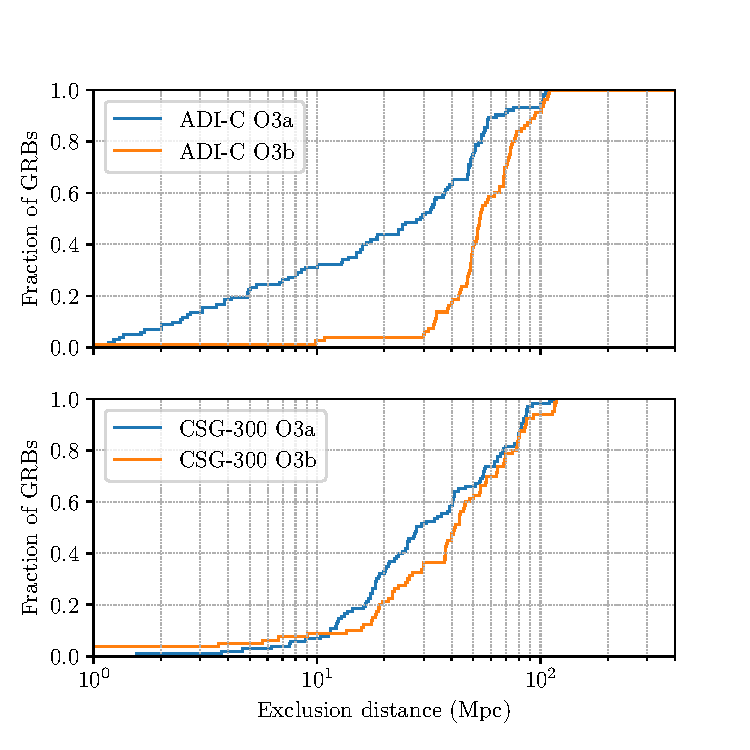
\includegraphics{figures/grb/compare-o3a.pdf}
  \caption
	[Cumulative distributions of O3a and O3b exclusion distances for the ADI-C (top) and 300-Hz sine-Gaussian (bottom) waveforms.]
	{Cumulative distributions of O3a and O3b exclusion distances for the ADI-C (top) and 300-Hz sine-Gaussian (bottom) waveforms.
	These show the greatest improvement between O3a and O3b among their respective waveform sets.}
  \label{fig:grb-o3b-compare-o3a}
\end{figure}

Considering that longer-duration waveforms see greater improvement, the most obvious likely contributor is the implementation of autogating.
However, autogating cannot account for the changes in the $D_{90}$ of short-duration models.
These can only be explained by better GW detector sensitivity and/or reduced rates of short-duration glitches that overlap the injected signal.
Such glitches cause the entire injection to be vetoed, so it is not recovered by the search pipeline.
In particular, glitches caused by low-frequency scattering noise (discussed in Section~\ref{sec:vib}) can pepper a stretch of time with short-duration glitches, overlapping injections made at multiple points.
A method for reducing the occurrence of these glitches, \ac{RC} tracking, was implemented at for O3b, on Jan 7, 2020 at \ac{LLO} and Jan 15, 2020~\citep{Soni_2020}.

\begin{figure}[h]
  \centering
  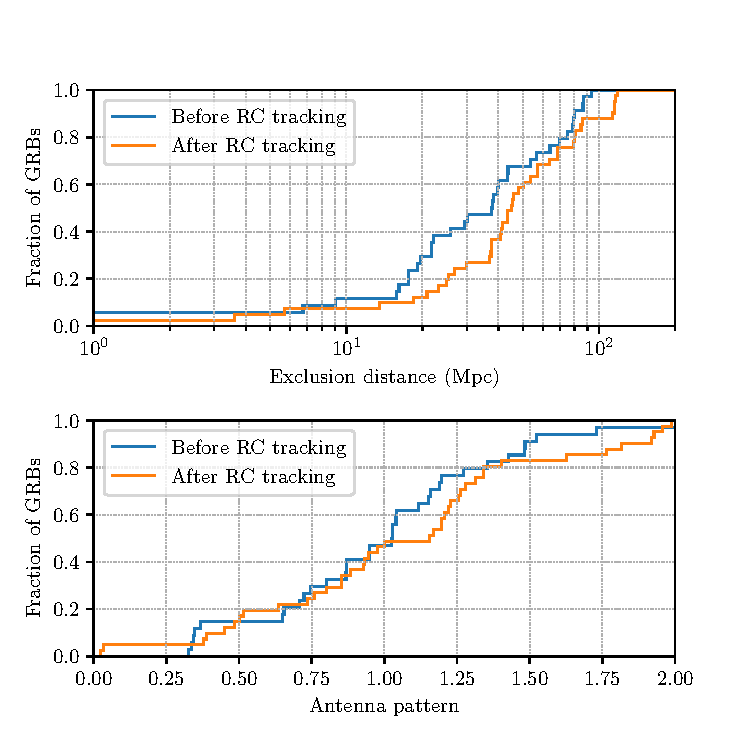
\includegraphics{figures/grb/compare-rc.pdf}
  \caption
	{Cumulative distributions of CSG-300 Hz exclusion distances (top) and the detector network antenna factors (bottom) for GRBs before and after the implementation of RC tracking.}
  \label{fig:grb-o3b-compare-rc}
\end{figure}

Figure~\ref{fig:grb-o3b-compare-rc} gives evidence for the effect of glitch mitigation on \xpip sensitivity.
Although there is clearly a bias towards higher antenna responses after RC tracking, they do not entirely account for the huge substantial increase in exclusion distances.

In summary, noise mitigation is a crucial part of improving the sensitivity of the generic transient search.
As discussed above, there may plenty that can be inferred even in the absence of detections.
Better detector sensitivities in \ac{O4}, along with the development of new glitch subtraction methods, could allow more confident exclusion of GW emission models, or some regions of their parameter space, associated with GRBs.


\subsection{Model exclusion}\label{sec:grb-o3b-models}

Although \xpip is an entirely unmodeled \ac{GW} search pipeline, given the substantial improvement in the exclusion distances in O3b, we may be approaching the point at which extreme GW emission models associated with long GRBs can be excluded using our null results and the sensitivity estimates for injected waveforms.
Using detection efficiency curves of both the O3a and O3b searches, we can compute for each model an exclusion confidence using the method described in~\citet{Kalmus_2013} for supernova searches~\citep{burst_o2}.
The model exclusion probability given $N$ targeted GRBs is

\begin{equation}
	P_{\text{excl}} = 1 - \prod_{i=1}^N \left[ 1 - \varepsilon_i(d_i) \right]
\end{equation}
where $\varepsilon_i(d_i)$ is the detection efficiency at the source distance of $d_i$.
Of the 86 GRBs analyzed in the O3b search by \xpip, only one, GRB 191221B has a redshift measurement (GRB 200205B did not occur at a time when at least two detectors were active and was therefore not included).
For the remaining GRBs, we have no distance measurement, but instead we can sample $d_i$ from the historical distribution of redshifts measured by Swift \ac{BAT} since 2005.

\begin{figure}[h]
  \centering
  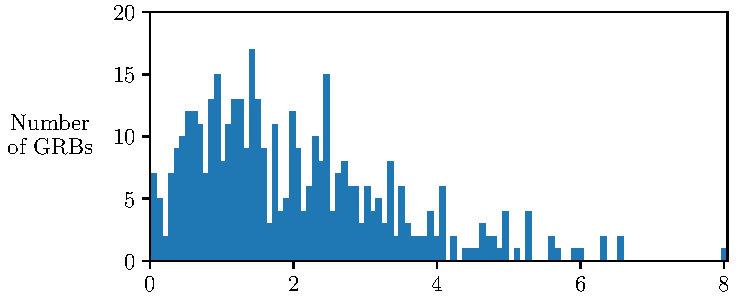
\includegraphics{figures/grb/redshifts.pdf}
  \caption{Histogram of redshift measurements for GRBs detected by Swift BAT.}
  \label{fig:grb-o3b-redshifts}
\end{figure}

The Swift GRB archive has redshift measurements for 411 triggers~\citep{swift_archive}.
Figure~\ref{fig:grb-o3b-redshifts} shows the distribution of those measurements, from which we sample distances for the 86 GRBs analyzed, using inverse transform sampling, and compute exclusion probability for each model.
This is repeated 1,000 times and $P_{\text{excl}}$ is averaged for each model across all trials.

\begin{table}[h]
  \hspace{0.5cm}
  \caption
  {\label{tab:grb-o3b-model-exclusion} Exclusion confidence for each injected waveform model.}
  \begin{tabular}{c c c c c}
    \hline
    \hline
    \rule{0pt}{4ex}
    & CSG 70\,Hz & CSG 100\,Hz & CSG 150\,Hz & CSG 300\,Hz \\
    \hline
    \rule[-2ex]{0pt}{4ex}
		$P_{\text{excl}}$ & \textbf{0.74} & \textbf{0.63} & 0.44 & 0.12
  \end{tabular}
  %
  \begin{tabular}{c c c c c c}
    \hline
    \hline
    \rule{0pt}{4ex}
    & ADI-A & ADI-B & ADI-C & ADI-D & ADI-E \\
    \hline
    \rule[-2ex]{0pt}{4ex}
    $P_{\text{excl}}$ & 0.04 & \textbf{0.61} & 0.15 & 0.00 & 0.18 \\
    \hline
  \end{tabular}
\end{table}

The averages are presented in Table~\ref{tab:grb-o3b-model-exclusion}.
The model with the highest exclusion probability is the 70-Hz sine-Gaussian model.
Assuming that the Swift redshift distribution is representative of the GRBs analyzed by \xpip, it is more likely than not that we can rule out the very optimistic energies simulated by the low-frequency 70-Hz and 100-Hz sine-Gaussian injections ($E_{\text{GW}} = 10^{-2}\,\msol c^2$) based on the lack of GW-GRB joint detections at O3 sensitivity.

If the sensitivity of the LIGO detectors continues to improve in \ac{O4}, we may well be able to begin ruling out the most extreme emission models.
The exclusion probability for the ADI-B model is 0.61, making it the only unfavorable ADI model so far.
This accretion disk instability model is simulated for a central \ac{BH} mass of $M=10\,\msol$, a dimensionless spin parameter of $\chi=0.95$, and a very large clump mass of $\epsilon=0.2$ times that the central \ac{BH}.
It is the most extreme of the ADI models, and it would not be surprising to see it being ruled out in future searches.

{\color{red}More to be added to this section. Some work is still ongoing.}
